%%
%% The original source files were:
%%
%% samples.dtx  (with options: `all,proceedings,bibtex,manuscript')
%% 
%% IMPORTANT NOTICE:
%% 
%% For the copyright see the source file.
%% 
%% Any modified versions of this file must be renamed
%% with new filenames distinct from sample-manuscript.tex.
%% 
%% For distribution of the original source see the terms
%% for copying and modification in the file samples.dtx.
%% 
%% This generated file may be distributed as long as the
%% original source files, as listed above, are part of the
%% same distribution. (The sources need not necessarily be
%% in the same archive or directory.)
%%
%%
%% Commands for TeXCount
%TC:macro \cite [option:text,text]
%TC:macro \citep [option:text,text]
%TC:macro \citet [option:text,text]
%TC:envir table 0 1
%TC:envir table* 0 1
%TC:envir tabular [ignore] word
%TC:envir displaymath 0 word
%TC:envir math 0 word
%TC:envir comment 0 0
%%
%% The first command in your LaTeX source must be the \documentclass
%% command.
%%
%% For submission and review of your manuscript please change the
%% command to \documentclass[manuscript, screen, review]{acmart}.
%%
%% When submitting camera ready or to TAPS, please change the command
%% to \documentclass[sigconf]{acmart} or whichever template is required
%% for your publication.
%%
%%
\documentclass[manuscript,screen,review]{acmart}
% Chinese body (compile with XeLaTeX / LuaLaTeX)
\usepackage[UTF8,scheme=plain]{ctex}


\usepackage{algorithm}
% Use algorithmicx + algpseudocode: provides \Require, \Ensure, \State, and \Comment
\usepackage{algorithmicx}
\usepackage{algpseudocode}
% Provide compatibility shims for uppercase macros used in the document
% Some authors use \REQUIRE/\ENSURE/\UPON/\ENDUPON (uppercase) — map them to algpseudocode
\providecommand{\REQUIRE}[1]{\Require{#1}}
\providecommand{\ENSURE}[1]{\Ensure{#1}}
% \UPON{<cond>} will render as a bold 'Upon <cond>' state line inside algorithmic blocks
\providecommand{\UPON}[1]{\State\textbf{Upon}~#1}
\providecommand{\ENDUPON}{}
\providecommand{\Upon}[1]{\State\textbf{Upon}~#1}
\providecommand{\EndUpon}{}
% Provide uppercase aliases commonly used in algorithm blocks
\providecommand{\STATE}{\State}
\providecommand{\COMMENT}[1]{\Comment{#1}}
% Map common uppercase algorithmic keywords to algorithmicx/algpseudocode commands
\providecommand{\IF}{\If}
\providecommand{\ELSE}{\Else}
\providecommand{\ELSIF}{\ElsIf}
\providecommand{\ENDIF}{\EndIf}
\providecommand{\FOR}{\For}
\providecommand{\ENDFOR}{\EndFor}
\providecommand{\WHILE}{\While}
\providecommand{\ENDWHILE}{\EndWhile}
\providecommand{\RETURN}{\State\textbf{return}~}
\usepackage{tikz}
% Load common tikz libraries used in figures (positioning provides the "of" syntax)
\usetikzlibrary{positioning,arrows.meta,calc,shapes,shadows}
% color support for \textcolor used inside algorithms
\usepackage{xcolor}
% Math packages required for \text and bold symbols inside math
\usepackage{amsmath}
\usepackage{bm}
\usepackage{adjustbox}
% Define common math operators used in the document
\DeclareMathOperator*{\argmin}{arg\,min}
\DeclareMathOperator*{\argmax}{arg\,max}
\usepackage{multirow}
\usepackage{booktabs}
% Enable list customization (leftmargin, itemsep, etc.) used in the document
\usepackage{enumitem}
\newlength{\tblwidth}
\setlength{\tblwidth}{\linewidth}
% Ensure header height is sufficient for fancyhdr
\setlength{\headheight}{20.48303pt}
% theorem environments used in the document
\usepackage{amsthm}
\newtheorem{theorem}{Theorem}
\newtheorem{definition}{Definition}
\newtheorem{assumption}{Assumption}
\newtheorem{proposition}{Proposition}
\newtheorem{problem}{Problem}
\newtheorem{lemma}{Lemma}
\newtheorem{corollary}{Corollary}
\newtheorem{remark}{Remark}

\newenvironment{tablenotes}{%
    \par\footnotesize
    \begin{list}{}{% 
        \setlength{\leftmargin}{1.5em}%
        \setlength{\labelsep}{0.5em}%
        \setlength{\itemsep}{0pt}%
        \setlength{\parsep}{0pt}%
    }%
}{%
    \end{list}%
}

%%
%% \BibTeX command to typeset BibTeX logo in the docs
\AtBeginDocument{%
  \providecommand\BibTeX{{%
    Bib\TeX}}}

%% Rights management information.  This information is sent to you
%% when you complete the rights form.  These commands have SAMPLE
%% values in them; it is your responsibility as an author to replace
%% the commands and values with those provided to you when you
%% complete the rights form.
\setcopyright{acmlicensed}
\copyrightyear{2025}
\acmYear{2025}
\acmDOI{XXXXXXX.XXXXXXX}

%% These commands are for a PROCEEDINGS abstract or paper.
%%  \acmConference[Conference acronym 'XX]{Make sure to enter the correct
%% 	conference title from your rights confirmation email}{June 03--05,
%% 	2018}{Woodstock, NY}

%%
%%  Uncomment \acmBooktitle if the title of the proceedings is different
%%  from ``Proceedings of ...''!
%%
%%\acmBooktitle{Woodstock '18: ACM Symposium on Neural Gaze Detection,
%%  June 03--05, 2018, Woodstock, NY}
%%\acmISBN{978-1-4503-XXXX-X/2018/06}


%%
%% Submission ID.
%% Use this when submitting an article to a sponsored event. You'll
%% receive a unique submission ID from the organizers
%% of the event, and this ID should be used as the parameter to this command.
%%\acmSubmissionID{123-A56-BU3}

%%
%% For managing citations, it is recommended to use bibliography
%% files in BibTeX format.
%%
%% You can then either use BibTeX with the ACM-Reference-Format style,
%% or BibLaTeX with the acmnumeric or acmauthoryear sytles, that include
%% support for advanced citation of software artefact from the
%% biblatex-software package, also separately available on CTAN.
%%
%% Look at the sample-*-biblatex.tex files for templates showcasing
%% the biblatex styles.
%%

%%
%% The majority of ACM publications use numbered citations and
%% references.  The command \citestyle{authoryear} switches to the
%% "author year" style.
%%
%% If you are preparing content for an event
%% sponsored by ACM SIGGRAPH, you must use the "author year" style of
%% citations and references.
%% Uncommenting
%% the next command will enable that style.
%%\citestyle{acmauthoryear}


%%
%% end of the preamble, start of the body of the document source.
\begin{document}

%%
%% The "author" command and its associated commands are used to define
%% the authors and their affiliations.
%% Of note is the shared affiliation of the first two authors, and the
%% "authornote" and "authornotemark" commands
%% used to denote shared contribution to the research.
\author{Qi Yu}
%%\authornote{.}
%%\authornotemark[1]
\email{230240012@seu.edu.cn}
%%\orcid{1234-5678-9012}
\affiliation{%
	\institution{School of Cyber Science and Engineering, Southeast University}
	\city{Nanjing}
	\state{Jiangsu}
	\country{PR China}
}


\author{Wei Li}
%%\orcid{1234-5678-9012}
\email{xchlw@seu.edu.cn}
\authornote{corresponding author}
%%\authornotemark[1]
\affiliation{%
	\institution{School of Computer Science and Engineering, Southeast University}
	\city{Nanjing}
	\state{Jiangsu}
	\country{PR China}
}


%%
%% By default, the full list of authors will be used in the page
%% headers. Often, this list is too long, and will overlap
%% other information printed in the page headers. This command allows
%% the author to define a more concise list
%% of authors' names for this purpose.

%%\renewcommand{\shortauthors}{Yu et al.}

\title{基于耦合互证与可问责沉默的被劫持设备任务状态伪造检测}
\subtitle{Detecting Task-State Falsification by Compromised Devices via Coupled Corroboration and Accountable Silence}

\renewcommand{\shortauthors}{Yu and Li}

\begin{CCSXML}
<ccs2012>
 <concept>
  <concept_id>10002978.10003006.10003013</concept_id>
  <concept_desc>Security and privacy~Intrusion detection systems</concept_desc>
  <concept_significance>500</concept_significance>
 </concept>
 <concept>
  <concept_id>10010583.10010662.10010674</concept_id>
  <concept_desc>Hardware~Safety critical systems</concept_desc>
  <concept_significance>300</concept_significance>
 </concept>
 <concept>
  <concept_id>10003033.10003083.10003095</concept_id>
  <concept_desc>Networks~Cyber-physical networks</concept_desc>
  <concept_significance>300</concept_significance>
 </concept>
</ccs2012>
\end{CCSXML}

\ccsdesc[500]{Security and privacy~Intrusion detection systems}
\ccsdesc[300]{Hardware~Safety critical systems}
\ccsdesc[300]{Networks~Cyber-physical networks}

\begin{abstract}
被劫持的现场设备可以如实上报物理量，而仅伪造离散的任务状态；此类伪造不产生物理残差，因而残差检测、过程一致性检验与虚假数据注入检测等以单一观测者为前提的方法，在原理上即无法将其检出（看门狗只能发现完全沉默，无法判别内容真伪）。
已有文献指出了事件触发通信下的沉默攻击面；见证式位置证明多按地理邻居选取见证者，工业心跳机制则仅表征通信活性。现有工作仍缺少两项能力：一是借助\textbf{任务耦合的对端设备}否证完成类虚假声明，二是在\textbf{不依赖共识分歧}的前提下对沉默行为作出确定性归责。
本文提出两条互补的检测通道：在任务图导出的 $O(1)$ 规模见证集上进行耦合互证，以及由哈希链锚定的可问责沉默（accountable silence，即将设备``停止上报''这一行为本身变为可确定性归因的事件）。在互证超图 $H$ 上\textbf{存在对端设备的交接环节}，两通道合用后攻击策略 P1--P3 均不存在可行的获胜分支；在缺乏对端设备的覆盖缺口上，P3 仍可规避检测；一跳串谋（P4）仅延迟判定时刻。心跳间隔 $T_{\mathrm{hb}}$ 由安全时间预算反向求解确定，而非人为选取。
串谋代价由互证超图上前向可达闭包的基数量化（中位数为 5，最坏情形为 1）；检测时延的无条件上界 $r\,T_{\mathrm{hb}}$ 与危害模型导出的时间预算相衔接（相应定理仅适用于沉默通道，运动危害仅用于校准预算量级）。
在 Fischertechnik Trier 工业物联网事件日志上的实验表明：在协议其余部分不变、仅替换见证选取策略时，空间邻居策略只恢复约 52\% 的检出率；对于伪报完成且维持心跳的 P3，仅耦合互证有效；在 $n{=}28$ 的对照规模下，最严格预算口径下的心跳带宽约为 7.7\,KB/s，约为 5\,Hz 全网 PBFT 的 $1/131$。
\end{abstract}

\keywords{任务状态伪造, 耦合互证, 可问责沉默, 工业调度, 被劫持设备, 带宽--安全权衡}

\maketitle

%=============================================================================
\section{引言}
\label{sec:introduction}

\subsection{研究背景与动机}

工业生产调度系统由中央调度器与一组异构现场设备构成：设备执行下行命令并上报上行状态，派工决策依赖调度器维护的\textbf{任务状态视图}。
因此，攻击面在于污染该视图以诱导调度器派工，而非攻破设备的连续控制回路。
被劫持设备可以如实上报位置与运动学量，仅将``完成''、``可用''等离散结果位篡改为真——此类\textbf{任务状态伪造}不产生物理残差，残差类虚假数据注入（false data injection, FDI）检测、数字孪生 KPI 异常检测与单观测者的计划一致性检验对其均在原理上失效。

下面五点刻画了这一问题的结构：第一点解释伪造为何对单观测者不可见，其余四点给出可被检测机制利用、而攻击者难以同时伪造的结构。
其一，离散任务状态可在不产生物理残差的情况下被伪造，单观测者可见的字段甚至能够与良性样本逐字段一致。
其二，任务交接是\textbf{由双方共同参与的物理事件}：交付是否真实发生，其证据存在于诚实对端设备的到料、取件等本地传感中，攻击者无法控制。
其三，合格见证者由\textbf{任务图}而非无线拓扑决定，见证集规模为 $O(1)$，且在任务下发时即已确定。
其四，在事件触发语义下，``未收到完成消息''可被调度器按预测继续推进，沉默本身因而不产生代价——除非原像缺失被预先承诺为可归因事件（该承诺仅约束会话在线状态，不涉及结果位的真伪）。
其五，互证的待决（pending）状态由下行命令打开，而非由完成声明打开；伪造的任务状态若要维持到物料被消耗，攻击者须控制任务链上的整个前向可达闭包。

\subsection{与已有工作的差距}

单观测者残差与 FDI 方向的工作假定伪造必然扰动连续物理量~\cite{ditof2024,dtmpc2025}；PeerReview 明确指出其无法对``应发送而未发送''作确定性归责~\cite{peerreview2007}；Polygraph 与 ABC 的归责以共识分歧已经发生为前提~\cite{polygraph2021,abc2023}；TESLA 声明其不提供不可否认性~\cite{tesla2001,rfc4082}；IEC 61850 GOOSE 心跳仅表征通信活性；COLAW 与 Vouch+ 等位置证明按地理邻居选取见证者~\cite{colaw2020,vouch2019}；DIAT 等方案依赖 TEE 与软件完整性度量~\cite{diat2019}。
现有工作尚未解决的问题是：如何借助任务耦合的对端设备否证离散的完成声明，以及如何在不依赖共识分歧的前提下对沉默行为作出归责。

\subsection{本文方法}

考虑 AGV--机械臂车间场景：调度器命令 AGV-7 将工件运送至机械臂 R3 完成交接。
AGV-7 已被劫持，其目标是伪报``任务已完成、当前空闲''，以持续获取派工。
攻击者可选的策略共四类：（P1）伪报完成且不维持心跳；（P2）完全沉默，即不再发送任何上行消息；（P3）伪报完成但按时披露心跳原像；（P4）与下一跳对端设备串谋（collusion），使其为伪造的交接提供虚假确认。
针对上述四类策略，本文设计两条互补的检测通道：耦合互证处理完成类声明，可问责沉默处理心跳原像。
两条通道各自存在对方无法覆盖的缺口：\textbf{仅使用沉默通道}无法检出按时披露原像的伪报（P3）；\textbf{仅使用互证通道}虽可借助命令开启的互证窗口，对存在对端设备的沉默作超时检出（以全部活动为分母时并非全部检出），但其时延受派发排队支配（数十至数百秒），无法给出无条件的安全时延上界。
\textbf{两者合用}后，在存在对端设备的交接环节上 P1--P3 均不存在可行的获胜分支：伪报被对端设备否证，沉默因原像缺失而在秒级内被判定；按时披露原像但仍伪报完成（P3）只能由耦合互证检出。
在缺乏对端设备的覆盖缺口上互证通道失效，若 P3 同时维持心跳，则该分支仍可规避检测（第~\ref{sec:covdesign}~节）。
一跳串谋（P4）仅延迟判定时刻，其代价由前向可达闭包的基数 $k$ 度量。
本文以该场景阐明威胁模型；实验则在 Fischertechnik Trier 日志上实例化同一组形式化对象（该日志不含 AGV 与通信层数据，心跳与危害预算参数的来源另行标注）。
图~\ref{fig:attack-tree} 概括了上述四类攻击策略及其对应的检出通道。

\begin{figure}[t]
  \centering
  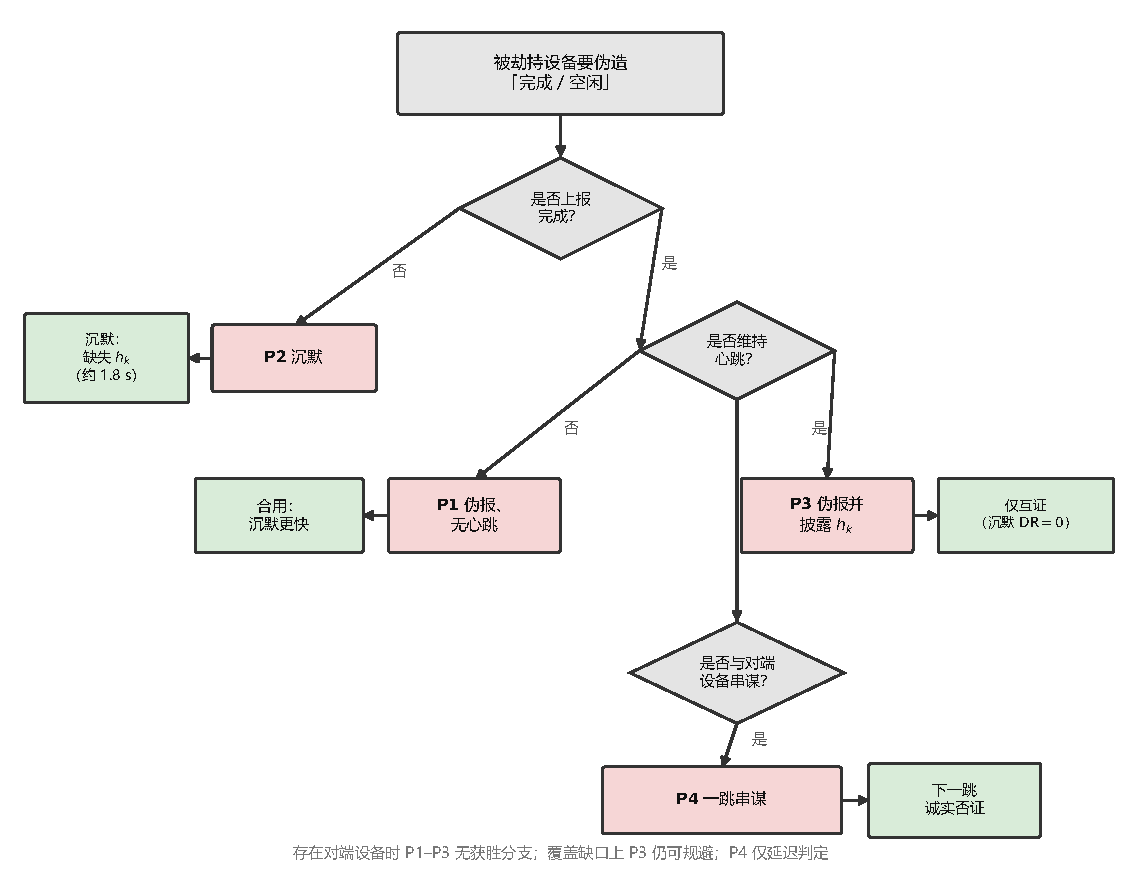
\includegraphics[width=\columnwidth]{fig/fig_attack_tree_CN.pdf}
  \Description{Attacker decision tree with branches P1--P4 and detecting mechanisms.}
  \caption{攻击者决策树（P1--P4）。存在对端设备时，两通道合用后 P1--P3 均无可行的获胜分支；在覆盖缺口上 P3 仍可规避检测；P4 仅延迟判定时刻。}
  \label{fig:attack-tree}
\end{figure}

\subsection{主要结果}

在 Fischertechnik Trier 工业物联网事件日志上：在协议其余部分不变、仅替换见证选取策略时，空间邻居策略只恢复约 52\% 的检出率；对于伪报完成且维持心跳的 P3，仅耦合互证有效；在 $n{=}28$ 的对照规模下，最严格预算口径下的心跳带宽约为 7.7\,KB/s，约为 5\,Hz 全网 PBFT 的 $1/131$。
存在对端设备时，两通道合用后 P1--P3 均不存在可行的获胜分支；在缺乏对端设备的覆盖缺口上，P3 仍可规避检测。

\subsection{贡献}

问题设定（无残差的任务状态伪造）用于界定研究范围，不单独计为技术贡献。本文的技术贡献有三点：
\begin{enumerate}[leftmargin=*,itemsep=2pt]
  \item \textbf{耦合互证的见证选取原则与串谋界。} 见证集由任务图诱导的互证超图导出；在协议其余部分不变、仅替换见证选取策略时，空间邻居策略只恢复约 52\% 的检出率，且所需见证集规模更大，说明性能增量来自选取原则本身，而非仅仅``引入了见证者''。
  \item \textbf{可问责沉默。} 以一次签名锚定的哈希链与有界心跳相结合，将原像缺失转化为不依赖共识分歧的确定性归因（所归责的是``应披露而未披露''，而非``结果位为真''）。
  \item \textbf{带宽--安全裕度权衡。} 推导链条为：危害模型 $\to$ 时间预算 $\to$ 可行的 $(r,T_{\mathrm{hb}})$ $\to$ 带宽下界；相应定理仅衔接沉默通道的无条件时延上界 $r\,T_{\mathrm{hb}}$。运动碰撞危害仅用于校准预算量级，主要安全论断仍是调度损害下的可检测性。
\end{enumerate}
非对称密码开销的控制（高频路径使用 MAC 与哈希链，仅在稀有事件中使用数字签名）属于工程实现层面的附带结果，不作为主要创新点。

本文余下部分安排如下：第~\ref{sec:related}~节界定相关工作的范围；第~\ref{sec:model}~节给出问题描述、威胁模型与覆盖矩阵；第~\ref{sec:method}~节描述方法（含串谋界与带宽定理）；第~\ref{sec:eval}~节报告实验结果；第~\ref{sec:conclusion}~节给出结论、局限与未来工作。命题~\ref{prop:nr}~的归约证明见附录~\ref{app:nr}。

%=============================================================================
\section{相关工作}
\label{sec:related}

\subsection{事件触发通信与沉默攻击面}

在 PISTIS 等事件触发的实时拜占庭协议中，``事件''指消息到达与连通性变化~\cite{pistis2021}；控制论方向的工作则以连续状态偏差超过阈值作为触发条件~\cite{tac2025el,hdetm2024}。
工业领域的轻量 PBFT 工作多致力于压缩单轮消息数 $M$ 与协议阶段数~\cite{ccgridw2023pbft,sensors2024aloha}，而共识频率 $R$ 仍由外部周期决定。
本文所指的事件位于工艺与任务语义层，不将``事件触发结合拜占庭容错''或降低共识频率 $R$ 作为创新点。
PISTIS 并不以任务语义事件作为输入，不宜作为本数据集上的数值基线；因此，协议其余部分保持一致的对照实验改由见证选取策略族（第~\ref{sec:tier2}~节）实现。

已有文献提出并分析了利用触发机制本身的非触发型恶意行为（non-triggering misbehavior）~\cite{nontrigger2022}：受损智能体虽已偏离期望状态，却不产生触发事件；相关工作亦在事件触发框架内开展抗欺骗控制器综合~\cite{asjc2023contain,ijrnc2023deception}。
上述工作止步于性能分析与鲁棒控制补偿，未给出``该段沉默是否合法''的可验证判定。
\textbf{该攻击的学术提出权归属上述文献}；本文的贡献在于离散任务调度语境下的运行时检出与归责。

\subsection{可问责性、哈希链与工业心跳}

PeerReview 提供通用的可问责层，但其明确指出无法对``应发送而未发送''作确定性揭发~\cite{peerreview2007}。
Polygraph 与 ABC 在分歧已经发生时输出不可反驳的证据~\cite{polygraph2021,abc2023}。
TESLA 采用延迟密钥披露实现源认证，但声明不提供不可否认性~\cite{tesla2001,rfc4082}；后续的 Inf-TESLA 等工作仍沿用同一原语边界~\cite{inftesla2022}。
IEC~61850 GOOSE 心跳的语义为通信活性（MaxTime / TAL），不含密码学绑定，心跳丢失仅触发失效安全（fail-safe）动作~\cite{goose615}。
US-AID 等设备在场证明所证明的是设备的物理在场~\cite{usaid}；本文沉默通道所证明的是会话仍然在线（原像按槽披露），\textbf{并不}证明任务状态处于可行域内。
本文的增量在于：在松散时间同步与有界心跳假设下，利用预承诺哈希链将原像缺失转化为确定性的可归因行为，且不以共识分歧已经发生为前提。

\subsection{见证选取与任务状态伪造}

DIAT 等方案依赖 TEE 与软件完整性度量~\cite{diat2019}；COLAW 与 Vouch+ 由地理邻居对位置进行见证~\cite{colaw2020,vouch2019}；车联网协同感知同样强调多见证者冗余~\cite{etsi460}；DiToF 利用数字孪生偏差的相关性对 FDI 作分类~\cite{ditof2024}。
本文的见证者是任务耦合的物理对端设备，见证内容是离散状态迁移是否真实发生；见证集由任务图预先确定，串谋代价由前向可达闭包的基数量化。

AGV 数字孪生 KPI 检测、基于 LSTM 孪生的模型预测控制与电网 FDI 检测等工作~\cite{dtmpc2025,agvkpi2022,fdi2024frontiers}的共同前提，是由单一观测者对连续物理量作残差检测；亦有专利将事件触发与多 AGV 抗 FDI 路径跟踪相结合，但其目标是控制补偿而非归责~\cite{cn120578205b}。
如实上报位置、仅伪造任务状态的攻击不产生残差，因而对上述方法族具有结构性免疫——这正是本文标题强调``任务状态''的原因。

\begin{table}[t]
  \centering
  \caption{相关工作定位（摘要）}
  \label{tab:rw}
  \begin{tabular}{@{}llp{0.38\columnwidth}@{}}
    \toprule
    方法类 & 核心前提 & 相对本文的局限 \\
    \midrule
    残差 / FDI / 数字孪生 & 连续物理量出现异常 & 对无残差的任务伪造失效 \\
    GOOSE 式心跳 & 通信活性 & 无身份绑定，不支持归责 \\
    Polygraph / ABC & 共识分歧已发生 & 沉默而无分歧时不适用 \\
    地理邻居见证 & 按无线拓扑选取见证者 & 非任务耦合，$|W|$ 不可预知 \\
    \textbf{本文} & 任务图见证与原像心跳归责 & --- \\
    \bottomrule
  \end{tabular}
\end{table}

%=============================================================================
\section{问题描述与威胁模型}
\label{sec:model}

\subsection{系统构成与形式化对象}
\label{sec:sys}

中央调度器 $S$ 与现场设备集 $\mathcal{D}=\{d_1,\dots,d_n\}$ 经工业网络互联。
设备之间不进行自治协商：仅执行下行命令 $u$，并上报上行声明 $r$。
$S$ 维护命令账本 $c$（记录已下发且未撤销的命令）；该账本是调度器本身已有的产物，\textbf{不属于本文贡献}。
活动（即任务实例）记为 $a$；由工艺模型导出任务图 $G=(V,E)$，进而导出互证超图 $H$（其超边为跨设备类、同位置的交付--取件对），见证集 $W(a)$ 由 $H$ 唯一确定。
互证窗口 $\Delta$ 须足以容纳派发排队时延；心跳间隔 $T_{\mathrm{hb}}$ 与触发判定所需的连续缺失槽数 $r$ 由安全时间预算反向求解确定。

引导示例以 AGV 与机械臂的交接阐明语义，实验则以 Trier 数据集中的工位交接实例化同一组对象（表~\ref{tab:symbols}）；二者对应同一形式化系统，而非两套不同的系统。

\begin{table}[t]
  \centering
  \caption{形式化对象及其 Trier 实例化}
  \label{tab:symbols}
  \begin{tabular}{@{}llp{0.42\columnwidth}@{}}
    \toprule
    符号 & 含义 & Trier 数据集上的实例化 \\
    \midrule
    $S$ & 调度器 & 日志中的派工时刻 \\
    $\mathcal{D}$ & 设备实例 & \texttt{vgr\_1}、\texttt{hbw\_2}、\texttt{mm\_1} 等（共 15 个资源） \\
    $u$ & 下行命令 & \texttt{assigned} 字段、计划时长与起止位置 \\
    $c$ & 命令账本 & 由派工字段重建（非本文贡献） \\
    $a$ & 活动实例 & 合并后的活动记录 \\
    $G,H$ & 任务图 / 互证超图 & 16 个 BPMN 模型；185 条见证边 \\
    $W(a)$ & 见证集 & 中位数 $|W|{=}1$，最大值 6 \\
    $\Delta$ & 互证容差 & 260\,s（排队时延 p95 ${\approx}218$\,s） \\
    $T_{\mathrm{hb}},r$ & 心跳参数 & 由安全预算反向求解；回放口径为 $0.2$\,s / $9$ \\
    \bottomrule
  \end{tabular}
\end{table}

\begin{figure}[t]
  \centering
  
\includegraphics[width=\columnwidth]{fig/fig_system_CN.pdf}
  \Description{Scheduler issues commands that open corroboration pending; devices send completion reports and heartbeat preimages; counterparts confirm or refute.}
  \caption{系统构成与消息回环：下行命令打开互证待决项；完成类声明由耦合互证通道处理，心跳原像由可问责沉默通道处理。}
  \label{fig:system}
\end{figure}

\subsection{消息回环}
\label{sec:msg}

下行 $S\!\to\!d$：命令 $u$ 一经入账即打开互证待决项——即使设备此后完全沉默，命令的下发时刻依然被记录在案。
上行 $d\!\to\!S$ 的两类载荷分开处理：
\begin{enumerate}[leftmargin=*,itemsep=1pt]
  \item \textbf{任务完成类}（结果位、起止位置、时长）$\to$ 由耦合互证通道处理；
  \item \textbf{心跳原像类}（槽 $k$ 对应的哈希链元素）$\to$ 由可问责沉默通道处理。
\end{enumerate}
在事件触发语义下，``未收到完成消息''并不等于``未下发命令''；看门狗可以发现``应上报而未上报''，却无法判别``已上报但内容为伪造''。

\subsection{威胁模型}
\label{sec:threat}

\textbf{攻击者}为被劫持的现场设备 $d\in\mathcal{D}$，调度器 $S$ 本身不被攻破。
攻击者\textbf{能够}：任意伪造或扣留上行声明；如实使用物理定位结果（因而不产生残差）；掌握过程模型以及\textbf{发往本机的命令}（命令账本对接收方可见，该设定强于``攻击者只能猜测最可能的下一步''）；与其他设备串谋；造成随机丢包或突发丢包（影响误报统计口径，但不改变判定语义）。
攻击者\textbf{不能}：攻破 $S$ 或篡改命令账本；在物理世界中制造未发生的交接，使诚实对端设备``观测到''该事件；伪造其他设备的哈希链原像或承诺根；在松散时间同步成立的前提下否认槽截止时刻的判定结果。

\textbf{攻击目标}是使 $S$ 的任务状态视图与物理现实脱节（伪报完成或空闲、造成下游工位饥饿等）。本文考虑的主要危害是调度损害；运动碰撞仅用于校准危害预算的量级。

\textbf{根本的非对称性在于：}攻击者可以控制上行声明的内容及是否发送，但无法控制物理交接是否真实发生，也无法控制其他设备的原像披露与 $S$ 侧的证据归档。

\begin{assumption}[显式假设]
系统满足松散时间同步（同步误差计入时钟偏移上界 $\varepsilon$）；参与交接的设备\textbf{默认}具备到料、取件一类的本地传感能力（覆盖矩阵与第一档实验的互证列均按此口径统计）；``缺乏传感能力''与``缺乏对端设备''是两类不同的覆盖缺口（第~\ref{sec:corr}~节）；不假设可信执行环境（TEE）；发往本机的命令默认对该设备可见，即不考虑更弱的攻击者知识等级。
\end{assumption}

\subsection{攻击类型与检测通道覆盖矩阵}
\label{sec:coverage}

表~\ref{tab:coverage} 同时给出威胁分类、方法必要性论证与消融实验的设计依据。
表中数值来自 Trier 数据集上的注入实验（注入率 0.2，随机种子 42，互证容差 260\,s）。
\textbf{各行的统计基数（分母）不同，需分别理解：}P1/P3/P4 仅从存在实测对端设备的声明中抽取（分别为 363 / 363 / 375 条），因此合用通道的 DR${=}1.000$ 是条件检出率，而非系统覆盖率；P2 从全部声明中抽取（527 条），故仅互证通道的 DR${=}0.746$——缺失的约四分之一正对应缺乏对端设备的覆盖缺口。
互证列默认对端设备具备显式否证能力（即具备到料、取件传感）；不具备该传感能力时的统计口径见第~\ref{sec:corr}~节，不应与本表的 $1.000/54.6$ 混用。
表中沉默通道的时延采用检测回放口径 $r{=}9,\,T_{\mathrm{hb}}{=}0.2$\,s（中位数约 1.8\,s），该口径只满足突发丢包下的误报预算，\textbf{不}满足运动危害对应的 $0.60$\,s 检测预算；若需满足该预算，应改用表~\ref{tab:budget} 中最严格的参数点 $(r,T_{\mathrm{hb}})=(10,0.058\,\mathrm{s})$。
第~\ref{sec:bw}~节的预算求解给出另一组可行的 $(r,T_{\mathrm{hb}})$，两组口径不可混用。
表中每格数值为检出率 / 时延中位数（秒）。

\begin{table*}[t]
  \centering
  \caption{攻击类型与检测通道覆盖矩阵（DR / 时延中位数）。P1/P3/P4 的分母为存在对端设备的活动，P2 的分母为全部活动。}
  \label{tab:coverage}
  \begin{tabular}{@{}lllll@{}}
    \toprule
    攻击 & 看门狗 S1 & 仅耦合互证 & 仅可问责沉默 & \textbf{合用} \\
    \midrule
    P1 伪报完成且不维持心跳 & 0.000 & 1.000 / 54.6 & 1.000 / 1.8 & \textbf{1.000 / 1.8} \\
    P2 完全沉默 & 1.000 / 334 & 0.746 / 325 & 1.000 / 1.8 & \textbf{1.000 / 1.8} \\
    P3 伪报完成且按时披露原像 & 0.000 & \textbf{1.000 / 54.6} & \textbf{0.000} & \textbf{1.000 / 54.6} \\
    P4 一跳串谋 & 0.000 & 0.184 / 355$^{\dagger}$ & 0.000 & 0.184 / 355$^{\dagger}$ \\
    \bottomrule
  \end{tabular}
  \begin{tablenotes}
    \item $^{\dagger}$P4 的分母为主受害活动上的伪造声明；串谋方的后续交付仍被下游设备否证，该环节 DR 为 $0.750$。良性流上的误报率：耦合互证为 $2.25\%$，看门狗约为 $4.2\%$。P1/P3/P4 的注入仅抽取存在对端设备的声明，P2 抽取全部声明；合用列的 $1.000$ 为条件检出率，而非系统覆盖率。
  \end{tablenotes}
\end{table*}

\textbf{表~\ref{tab:coverage} 的要点如下：}
（1）P3 行最为关键——当攻击者在伪报完成的同时按时维持心跳时，沉默通道的 DR${=}0$，只有耦合互证能够检出（合用列的时延 $54.6$\,s 来自互证检出，而非秒级的沉默判定界）；在缺乏对端设备的覆盖缺口上互证同样失效，P3 仍可规避检测；
（2）P1/P2 说明沉默通道不可省略——存在对端设备时互证也能检出沉默，但以全部活动为分母时，仅互证通道的检出率只有 $0.746$；两通道合用可将时延压缩至约 1.8\,s；
（3）看门狗对 P2 有效、对 P1/P3/P4 检出为 $0$，说明其并非人为削弱的对照基线；
（4）P4 是本文明确承认的能力边界——一跳串谋仅延迟判定时刻，其代价由串谋界量化。
单观测者残差与一致性方法族对 P1/P3 的结构性零检出见第~\ref{sec:eval}~节第一档，该档用于说明问题性质，不与本表的四列作直接性能对比。

%=============================================================================
\section{耦合互证与可问责沉默}
\label{sec:method}

\subsection{框架总览}
\label{sec:arch}

方法实现为开源原型 TESSERA，其模块与代码一一对应：M1~\texttt{ingest} 重建活动与命令账本；M2~\texttt{taskgraph} 导出 $G\!\to\!H$ 与见证集 $W(a)$；M3~\texttt{corroborate} 执行在线互证；M4~\texttt{silence} 与 \texttt{crypto} 负责承诺根管理与心跳判定；M5~\texttt{coverage} 统计覆盖率与缺乏对端设备的区间；M6~\texttt{collusion} 计算前向可达闭包；M7~\texttt{budget} 求解可行的 $(r,T_{\mathrm{hb}})$。
其中 M1--M2--M5--M6--M7 离线执行；设备注册时以一次数字签名锚定哈希链承诺根。
在线阶段：命令打开待决项；完成类声明由 M3 处理，心跳槽由 M4 处理；任一通道告警即冻结相关派工。
\texttt{baselines.py} 与 \texttt{attacks.py} 仅用于评估，不参与在线运行路径。
总体数据流见图~\ref{fig:architecture}。

\begin{figure*}[t]
  \centering
  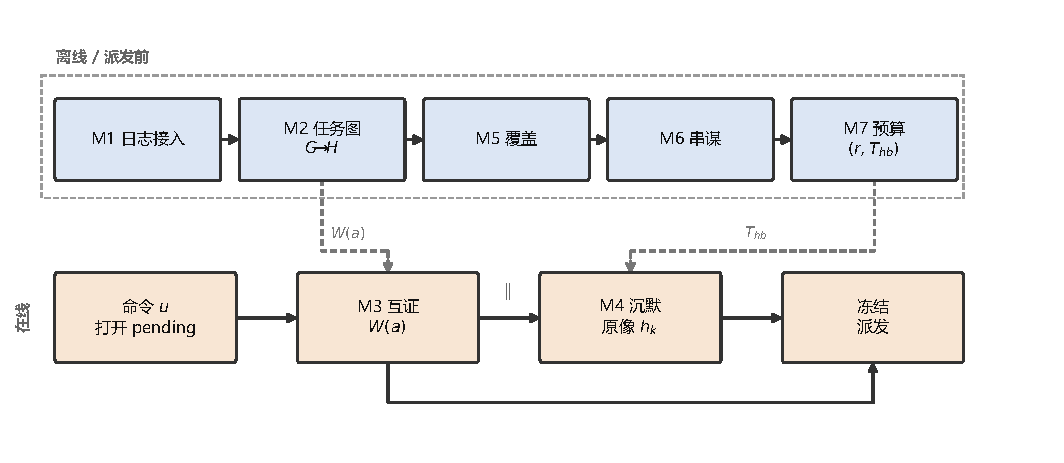
\includegraphics[width=0.92\textwidth]{fig/fig_architecture_CN.pdf}
  \Description{Offline modules M1--M7 and online corroboration parallel silence pipeline.}
  \caption{方法总体框架（M1--M7）。离线阶段导出见证集与参数 $(r,T_{\mathrm{hb}})$；在线阶段 M3 与 M4 并行运行、合用判定。}
  \label{fig:architecture}
\end{figure*}

\subsection{耦合互证}
\label{sec:corr}

由 BPMN 模型导出任务图 $G$，将跨设备类、同位置的交付--取件对构成互证超图 $H$；活动 $a$ 的见证集定义为
\[
  W(a)=\{d'\in\mathcal{D}: d'\text{ 与 }a\text{ 在 }H\text{ 上物理耦合}\}.
\]
在 Trier 数据集上共有 185 条见证边，$|W|$ 的中位数为 1，最大值为 6。
协议采用双截止时刻：看门狗截止时刻（自命令下发时刻起算）与互证截止时刻（对端设备确认窗口的终点），时序见图~\ref{fig:protocol}，判定过程见算法~\ref{alg:corr}。
判定结果为确认、显式否证或逾窗未决三者之一，相关证据以可转移的形式归档。
主表口径假定对端设备具备显式否证能力：P1/P3 中有 $349/363$ 条判定在取件时刻即已产生，时延中位数为 $54.6$\,s，远早于窗口到期。
若对端设备不具备到料、取件传感（棕地改造场景），则只能等待窗口超时，此时 P1 的检出率降至 $0.860$（$312/363$），时延中位数约为 $365$\,s。
可见传感覆盖度只影响互证时延，不改变见证选取原则。
\textbf{本文的贡献在于见证选取原则本身}：由于协议其余部分与见证选取相互独立，只需替换见证选取策略，即可在同一协议下与地理邻居、随机提名、全网询证以及 PBFT 式法定人数等方案作对照（第~\ref{sec:eval}~节第二档），从而将性能差异归因于选取原则。

互证时延受派发排队支配（本日志的排队时延 p95 约为 218\,s，故容差取 260\,s），因而该通道只能给出\textbf{条件}上界，其条件是对端设备已被派发；该上界不可代入功能安全时间预算。

\begin{figure}[t]
  \centering
  
\includegraphics[width=\columnwidth]{fig/fig_protocol_CN.pdf}
  \Description{Timeline of command-opened dual deadlines and heartbeat preimage slots.}
  \caption{协议时序：下行命令打开带双截止时刻的互证窗口；心跳槽与调度队列相互解耦。}
  \label{fig:protocol}
\end{figure}

\begin{algorithm}[t]
\caption{耦合互证（调度器侧）}
\label{alg:corr}
\begin{algorithmic}[1]
\Require 命令账本 $c$，互证超图 $H$，容差 $\Delta$
\Upon{收到下行派工 $u$ 并写入 $c$}
  \State 打开待决项 pending$(u)$；$W\!\leftarrow\!W(u)$；设定双截止时刻 $t_{\mathrm{wd}},t_{\mathrm{corr}}$
\EndUpon
\Upon{收到完成声明 $r$，或对端设备的确认或否证}
  \If{对端设备 $d'\!\in\!W$ 给出显式否证}
    \State 归档为 \textsc{Refuted}；冻结相关派工
  \ElsIf{在 $t_{\mathrm{corr}}$ 前收齐确认}
    \State 归档为 \textsc{Confirmed}
  \ElsIf{已超过 $t_{\mathrm{wd}}$ 或 $t_{\mathrm{corr}}$ 且声明已到达}
    \State 归档为 \textsc{Expired}（误报率分母仅统计此类）
  \EndIf
\EndUpon
\Upon{已超过 $t_{\mathrm{wd}}$ 且未收到完成声明}
  \State 归档为看门狗超时（计入 P2 检出；\textbf{不}计入互证误报率分母）
\EndUpon
\end{algorithmic}
\end{algorithm}

\subsection{可问责沉默}
\label{sec:silence}

本文所称``沉默''，指设备在应当披露心跳原像的槽上持续不发送上行消息；由链路故障引起的偶发丢包，则通过连续缺失阈值 $r$ 与误报预算加以区分。

设备以 Ed25519 签名注册承诺根 $R_d$，其绑定内容为 $\langle\mathrm{id},\,\mathrm{session},\,h_0,\,N,\,t_0,\,T_{\mathrm{hb}}\rangle$（其中 $t_0$ 与 $T_{\mathrm{hb}}$ 纳入签名范围，以防止设备事后修改心跳间隔而否认槽缺失）；哈希链满足 $h_k=H(h_{k+1})$，槽号与链元素一一对应，且协议拒绝提前披露 $h_{k+1}$（否则可由其推出 $h_k$，相当于为未来的沉默预先取得凭证）。
设备须在槽 $k$ 的截止时刻之前披露原像 $h_k$，其语义为``该设备在槽 $k$ 时刻仍维持本会话''（该凭证仅表示在线状态，\textbf{不}编码任务状态；见算法~\ref{alg:silence}）。
若连续 $r$ 个槽的原像缺失，即可确定性地判定为沉默。
完成类声明的真伪由耦合互证判定；原像仅证明消息来源，不证明结果位为真。
与 TESLA 的关键差别在于：链上原像直接作为一次性在线凭证使用，而非作为披露后即失效的 MAC 密钥。

\begin{algorithm}[t]
\caption{可问责沉默（调度器侧）}
\label{alg:silence}
\begin{algorithmic}[1]
\Require 已注册的承诺根 $R_d$，心跳间隔 $T_{\mathrm{hb}}$，判定阈值 $r$，时钟偏移上界 $\varepsilon$
\State 槽 $k$ 的截止时刻 $t_k^\star \leftarrow t_0 + k T_{\mathrm{hb}}+\varepsilon$
\Upon{到达时刻 $t_k^\star$}
  \If{已收到通过 $R_d$ 验证的原像 $h_k$}
    \State 重置缺失计数
  \Else
    \State 缺失计数 ${+}\!1$；若其 $\ge r$，则判定为可问责沉默并冻结派工
  \EndIf
\EndUpon
\end{algorithmic}
\end{algorithm}

\begin{proposition}[原像披露的不可否认性]
\label{prop:nr}
设（i）$R_d$ 由设备私钥对 $\langle\mathrm{id},\,\mathrm{session},\,h_0,\,N,\,t_0,\,T_{\mathrm{hb}}\rangle$ 签名锚定；（ii）槽号与链元素一一绑定，且协议拒绝提前披露；（iii）松散时间同步保证各接收方对截止时刻 $t_k^\star$ 的判定一致。
则任何持有 $(R_d,h_k)$ 的第三方均可验证``$h_k$ 只能由承诺者产生''（不可否认的是原像来源，而非任务状态为真）；而在截止时刻之后输出可通过验证的 $h_k'$，可归约为打破哈希函数 $H$ 的单向性或伪造 Ed25519 签名。
\end{proposition}
证明见附录~\ref{app:nr}。

由于心跳与调度队列相互解耦，$T_{\mathrm{detect}}\le r\,T_{\mathrm{hb}}$ 是\textbf{无条件}上界（在检测回放口径下，时延中位数约为 1.8\,s）；该上界即定理~\ref{thm:bw} 所使用的时延约束。

\subsection{两通道的合用与归因}
\label{sec:compose}

仅使用互证通道时：对存在对端设备的 P2，仍可因命令所开启的互证窗口超时而被检出，但以全部活动为分母的 DR 仅为 $0.746$，时延中位数达数百秒，且无法代入无条件的安全时间预算。
仅使用沉默通道时：P3 在按时披露原像的同时伪报完成，DR${=}0$——这直接说明耦合互证不可被替代。
两者合用后，\textbf{在存在对端设备的交接环节上} P1--P3 均不存在可行的获胜分支：P1/P2 的检测时延由沉默通道压缩至约 1.8\,s（回放口径，尚不满足运动危害对应的 $0.60$\,s）；P3 由耦合互证覆盖，其时延中位数 $54.6$\,s 来自互证检出，而非秒级的沉默判定界。
在缺乏对端设备的覆盖缺口上互证通道失效，若 P3 同时维持心跳，则该分支仍可规避检测。
P4 仅延迟判定时刻，详见覆盖矩阵。
两通道合用的第二个理由在于归因：沉默设备同时拒绝为上游设备提供确认，致使诚实上游的声明超时；沉默通道可直接判定出沉默设备，从而避免误冻结上游设备并对其重复核查（第~\ref{sec:ablation}~节给出 277/69 的实测结果）。

\subsection{覆盖缺口与串谋界的设计含义}
\label{sec:covdesign}

缺乏对端设备的区间（入库后无设备接手、同一设备原地完成多道工步、流程实例的末位活动等）在互证超图 $H$ 上不存在超边。
本实现\textbf{不}在在线运行路径中插入主动探测动作；理想传感预言机（sensing oracle，记为 U1，即假定任一交接均可被传感器观测的理想情形）给出的覆盖缺口上界约为 $29.95\%$（917 条），该值标识的是后续需要补足覆盖的目标区间，而非已部署的能力。
在这些区间上，针对完成类伪造的互证通道失效，只能由沉默通道保障活性：P1/P2 仍可因原像缺失被检出，而 P3 若维持心跳则该分支获胜。

串谋界还可反向用作派工约束：通过避免由任务图上不相邻的设备重复承接同一工件来增大 $k$，但该约束无法改变相邻工步由同一设备承接的情形。
表~\ref{tab:dispatch} 中的``可达理想''指在现有工艺路线可达范围内的最优排产，``无约束理想''指忽略工艺可达性的理论上限。
结果表明：在可达理想情形下，$k_{\min}$ 与中位数均保持不变，仅均值由 $5.13$ 提高至 $5.80$（约 $13\%$）；在 $1{,}282$ 条可改善的链中，原本 $k\le 2$ 的仅有 14 条，增益几乎全部落在本已安全的长链上。
无约束理想情形会将 $k_{\min}$ 高估为 2，而 23 条 $k{=}1$ 的链全部源于相邻工步由同一设备承接，无法通过排产调整消除。
因此该结果应定位为``在不牺牲产能的前提下改善 $k$ 的分布均值''，\textbf{不应}表述为提高了安全保证的下界；提高下界只能依靠引入原本不存在的见证事件。

\begin{table}[t]
  \centering
  \caption{串谋界用作派工约束的效果（Trier 数据集）}
  \label{tab:dispatch}
  \begin{tabular}{@{}lccc@{}}
    \toprule
     & 实际 & 可达理想 & 无约束理想 \\
    \midrule
    $k_{\min}$ & 1 & 1 & 2 \\
    $k$ 的中位数 & 5 & 5 & 6 \\
    $k$ 的均值 & 5.13 & 5.80 & --- \\
    \bottomrule
  \end{tabular}
\end{table}

\subsection{串谋界}
\label{sec:collusion}

\begin{definition}[下一跳对端设备与前向可达闭包]
\label{def:closure}
在互证超图 $H$ 上，活动 $a$ 的\textbf{下一跳对端设备}指与 $a$ 同处一条交付--取件超边、并实际接手该工件的设备。
从被伪造的活动出发，沿该关系迭代扩展，直至工件离开可互证的任务链，所得设备集合称为该起点的\textbf{前向可达闭包}，其基数记为 $k$。
伪造的任务状态能够维持到物料被消耗，当且仅当被劫持设备联盟覆盖了该闭包上的每一跳。
此处的形式化对象是闭包基数 $k$，而非将伪造声明与诚实观测者隔离所需的最小顶点割。
\end{definition}

统计作用域须保留由同一设备承接的 \textsc{SelfOnly} 链（228 条），否则将剔除全部 23 条 $k{=}1$ 的最坏情形样本；而同一流程实例内无设备接手的 \textsc{NoRealized} 链（183 条）属于覆盖缺口，不计入串谋界的分母。
表~\ref{tab:kdist} 与图~\ref{fig:collusion} 给出 $k$ 的分布：若要使任务状态伪造被永久隐藏，中位情形下需要五台设备同时被劫持，$81\%$ 的情形需要三台及以上，而最坏的 23 条链只需一台。
一跳串谋（P4）仅延迟判定时刻：主受害活动可因串谋方提供虚假确认而通过校验（DR 为 $0.184$），但串谋方的后续交付仍会被下游诚实设备否证（DR 为 $0.750$，即漏检率为 $25.0\%$）。
结构上 $k\le 2$ 的链约占 $19.0\%$，与该漏检率处于同一量级，二者可相互印证，但\textbf{不应}表述为定量吻合。

\begin{table}[t]
  \centering
  \caption{串谋界 $k$ 的分布（前向可达闭包；作用域内共 2\,373 条链）}
  \label{tab:kdist}
  \begin{tabular}{@{}lcccc@{}}
    \toprule
    $k_{\min}$ & 中位数 & 最大值 & $k\ge 3$ 占比 & $k{=}1$ 的最坏链 \\
    \midrule
    1 & 5 & 13 & $80.99\%$ & 23 \\
    \bottomrule
  \end{tabular}
\end{table}

\begin{figure}[t]
  \centering
  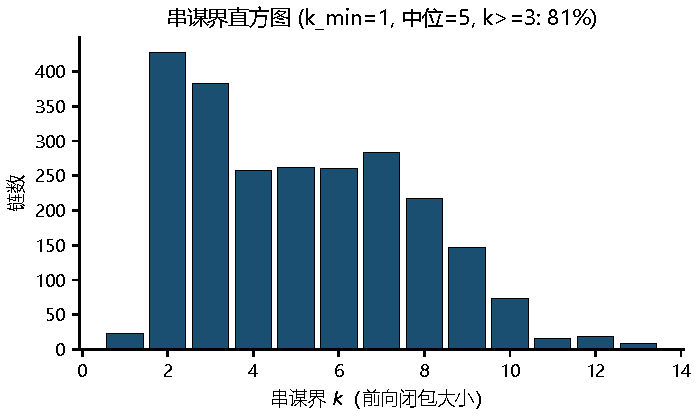
\includegraphics[width=\columnwidth]{fig/fig_collusion_CN.pdf}
  \Description{Histogram of collusion bound k over in-scope chains.}
  \caption{串谋界 $k$ 的分布（前向可达闭包；数据由原型 \texttt{tessera} 导出）。}
  \label{fig:collusion}
\end{figure}

\subsection{带宽--安全裕度权衡}
\label{sec:bw}

本节所界定的时延量取自沉默通道，即 $T_{\mathrm{detect}}\le r\,T_{\mathrm{hb}}$（互证窗口 $\Delta$ 由派发排队支配且无通用上界，不得代入）。
预算推导包含如下四个环节（图~\ref{fig:budget-chain}）：
\[
  \text{危害模型}\;\longrightarrow\;\text{时间预算}\;\longrightarrow\;(r,T_{\mathrm{hb}})\;\longrightarrow\;\text{带宽下界}.
\]

\begin{figure}[t]
  \centering
  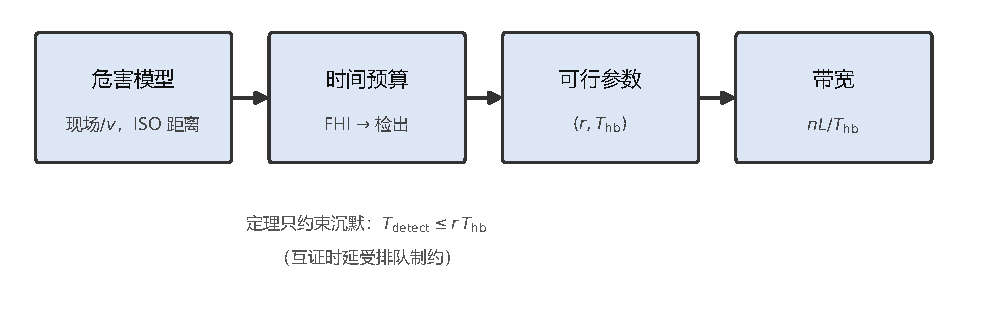
\includegraphics[width=\columnwidth]{fig/fig_budget_chain_CN.pdf}
  \Description{Four-stage chain from hazard model to bandwidth lower bound.}
  \caption{带宽--安全裕度的四环节推导链。相应定理仅衔接沉默通道的无条件时延上界。}
  \label{fig:budget-chain}
\end{figure}

若直接沿用汽车领域的故障处理时间间隔（fault handling interval, FHI）取值 $\mathrm{FHI}{=}2.43$\,s（DLR 算例~\cite{ase2023fhi}，其中反应段为 $0.25$\,s），将导致\textbf{虚假合规}：该口径留给检测的时间为 $2.18$\,s，而速度为 $1.5$\,m/s 的低速 AGV 在此期间将行驶 $3.27$\,m，达到 ISO~3691-4 算例中防护场 $1.275$\,m 的 $256\%$——此时车辆早已越出防护包络，而预算判据仍判定为满足。
防护场距离由 ISO~13855 的 $S{=}KT{+}C$ 与 ISO~3691-4 给出首段输入~\cite{iso13855,iso3691}（扫描仪响应 $0.10$\,s 与制动器响应 $0.15$\,s，对应反应距离 $0.375$\,m；叠加制动距离 $0.65$\,m 与安全裕度 $0.25$\,m，合计 $1.275$\,m）。
正确的衔接方式是由危害模型反推：$\mathrm{FHI}{=}\mathrm{field}/v{=}0.85$\,s，留给检测的时间为 $0.60$\,s，对应行驶距离 $0.90$\,m（为防护场的 $71\%$）。
当主要威胁为调度损害时，该换算仅用于校准预算量级，\textbf{不}构成本文的安全论断。

\begin{theorem}[带宽受安全约束限制]
\label{thm:bw}
给定设备数 $n$、单槽载荷 $L$、误报预算 $\Lambda$（单位：次/小时）与丢包模型（独立丢包，或以相关系数 $\rho$ 描述的突发丢包），
并设由危害模型导出的检测段预算为 $T_{\mathrm{budget}}$。
若存在整数 $r\ge 1$ 与 $T_{\mathrm{hb}}>0$，同时满足
（a）$r\,T_{\mathrm{hb}}\le T_{\mathrm{budget}}$，且
（b）在该丢包模型下由槽缺失引起的误报率 $\le\Lambda$，
则在满足（a）与（b）的前提下取最大的 $T_{\mathrm{hb}}$ 时，心跳带宽下界为 $B^\star=n L/T_{\mathrm{hb}}$。
若该最优点使条件（a）以等号成立而条件（b）仍有松弛，则称带宽受安全约束限制。
\end{theorem}
\begin{proof}[证明思路]
沉默判定至多等待 $r$ 个槽，故 $T_{\mathrm{detect}}\le r\,T_{\mathrm{hb}}$；要求其不超过 $T_{\mathrm{budget}}$ 即得条件（a）。
误报率由丢包导致的虚假缺失决定：独立丢包下，槽缺失次数服从二项分布，其尾概率为 $\Pr[X\ge r]$；突发丢包则通过相关系数 $\rho$ 提高有效连续丢包概率，从而提高满足 $\Lambda$ 所需的最小 $r$。
在可行集上最大化 $T_{\mathrm{hb}}$ 等价于最小化 $B=nL/T_{\mathrm{hb}}$。
最优点落在条件（a）的边界上，当且仅当安全预算比误报预算更为紧约束——这即是``带宽受安全约束限制''的可操作判据。
互证窗口 $\Delta$ 不在本定理范围内，因为它由派发排队支配且无通用上界。
\end{proof}

表~\ref{tab:budget} 给出设备数 28、丢包率 $1\%$、误报预算 1 次/小时条件下的求解结果。
四个口径中有三个受安全约束限制（余量 ${<}1.5\%$）；``汽车口径 + 突发丢包''则同时受安全与误报两条约束限制。
相对独立丢包，容忍突发丢包的带宽代价约为 $3.32$ 倍；预算由汽车口径收紧至运动危害口径时，带宽需求增加约 $4.59$ 倍。
本文报告最严格预算口径（运动危害 + 突发丢包）下的 $7{,}675$\,B/s，该值仍约为 5\,Hz 全网 PBFT 量级的 $1/131$；不采用最宽松的 $621$\,B/s，以避免夸大倍数优势。
参数来源见表~\ref{tab:params}：FHI、反应时间与丢包率均来自文献引用或仿真设定（Trier 日志不含 AGV 与通信层数据）。

\begin{table}[t]
  \centering
  \caption{带宽--安全裕度的可行参数点（$n{=}28$，$L{=}16$\,B，$\Lambda{=}1$ 次/h）}
  \label{tab:budget}
  \begin{tabular}{@{}llcccc@{}}
    \toprule
    危害口径 & 丢包模型 & $T_{\mathrm{hb}}$ & $r$ & 带宽 & 起作用的约束 \\
    \midrule
    汽车 $2.43$\,s & 独立 & $0.722$\,s & 3 & $621$\,B/s & 安全预算 \\
    汽车 $2.43$\,s & 突发 $\rho{=}0.3$ & $0.268$\,s & 8 & $1{,}672$\,B/s & 安全与误报 \\
    运动 $0.85$\,s & 独立 & $0.194$\,s & 3 & $2{,}311$\,B/s & 安全预算 \\
    运动 $0.85$\,s & 突发 $\rho{=}0.3$ & $0.058$\,s & 10 & $7{,}675$\,B/s & 安全预算 \\
    \bottomrule
  \end{tabular}
\end{table}

\subsection{复杂度与密码预算}
\label{sec:budget_eng}

每条完成声明需查询 $W(a)$（其规模中位数为 $O(1)$），并执行常数次验签与归档操作；每个心跳槽对应一次原像披露与一次哈希校验。
心跳带宽 $n L/T_{\mathrm{hb}}$ 由安全预算反向求解确定。
高频路径采用链路层认证与 MAC，可问责沉默采用哈希链令牌，仅在稀有事件与视图切换时使用数字签名。

%=============================================================================
\section{实验与结果分析}
\label{sec:eval}

\subsection{实验设置}
\label{sec:setup}

\textbf{主数据集：}Fischertechnik Trier IoT 事件日志与配套的 16 个 BPMN 模型~\cite{trier2022}，并自建 P1--P4 攻击注入器（默认注入率 0.2，随机种子 42）。
注入器的知识等级固定为 \texttt{ledger}：攻击者可见发往本机的命令，在伪造时如实回答与账本一致的字段，仅将结果位篡改为真；不设置更弱的知识等级，因为过弱的注入会使第一档的结构性零检出结论失真。
\textbf{场景、数据与参数的分离：}AGV 场景仅用于威胁说明；心跳参数、FHI 与丢包率均非本日志的实测值，其来源见表~\ref{tab:params}。
\textbf{评价指标：}检出率（DR）、误报率（FAR）、判别力（DR${-}${FAR}）、检测时延、见证集规模、串谋界 $k$、带宽以及未结算活动条数。
\textbf{对比公平性：}直接性能对比（第三档 H1）在等带宽或等误报率条件下进行；第二档实验保持协议其余部分一致、仅替换见证选取策略，不要求等带宽或等 FAR。
各基线按其\textbf{所消耗的信息}划分为四档（第一档至第四档），而非按文献出处分组。
W1 行中的 $\overline{|W|}$ 与本文相同，均为协议见证集均值 2.18，\textbf{不含}共识副本；其额外代价是全网共识消息带宽。
协议与各基线均实现于开源原型 TESSERA，复现入口见文末的数据与代码可用性说明。

\begin{table}[t]
  \centering
  \caption{预算与回放参数的取值来源（Trier 日志不含 AGV 与通信层数据）}
  \label{tab:params}
  \begin{tabular}{@{}llp{0.38\columnwidth}@{}}
    \toprule
    参数 & 取值 & 来源 \\
    \midrule
    $n$ & 28 & 引导示例规模，用于带宽对照 \\
    $L$ & 16\,B & 截断后的原像长度（实现取值） \\
    防护场 / $v$ & $1.275$\,m / $1.5$\,m/s & ISO~3691-4 算例~\cite{iso3691} \\
    汽车 FHI / $T_{\mathrm{react}}$ & $2.43$\,s / $0.25$\,s & ASE 算例~\cite{ase2023fhi} \\
    运动危害 FHI & $0.85$\,s & 由 $\mathrm{field}/v$ 得出（仅校准量级） \\
    $p$, $\rho$ & $1\%$, $0.3$ & 仿真设定，对应工业无线的成簇丢包 \\
    $\Lambda$ & 1 次/h & 误报预算（人为设定） \\
    回放 $T_{\mathrm{hb}},r$ & $0.2$\,s, $9$ & 在突发丢包口径下满足 $\Lambda$ \\
    互证容差 $\Delta$ & 260\,s & 良性流排队时延 p95 \\
    \bottomrule
  \end{tabular}
\end{table}

\subsection{第一档：单观测者方法的原理性失效}
\label{sec:tier1}

P1 的伪造声明在单观测者可见的 7 个字段上与良性样本逐字段一致，其时长 $100\%$ 落在对应（设备, 操作）组合的良性四分位距内。
因此，看门狗 S1、计划一致性残差 S2（通用 FDI 类方法）与对齐式过程一致性检验 S3 对 P1/P3 的失效是\textbf{原理性的}，而非阈值标定不当所致。
为排除``基线实现不充分''的质疑，本文作如下处理：所有阈值均在纯良性流上标定；看门狗采用与本文相同的窗口与 260\,s 容差；S3 不采用朴素的流程实例内相邻顺序判据（并发物料链、XOR 可选后继与不完整的 BPMN 模型会引入约 $28\%$ 的非攻击性误报），而仅保留全局非法活动与交接对上的严格逆序两类判据，修正后其 $\mathrm{FAR}{=}0$ 且 $\mathrm{DR}{=}0$。
R0 是告警率与上述基线相匹配的随机指控，用作性能下界参照。
在本档中 P1 与 P3 的结果必然相同（二者的差别仅在原像字段，而该字段对单观测者不可见）；P2 列如实反映了看门狗、残差与一致性方法同样能够发现沉默。
本档的互证列与覆盖矩阵采用相同的统计口径，即对端设备具备传感能力（P1/P3 的 DR${=}1.000$）；不具备传感能力时的结果见第~\ref{sec:corr}~节。
本档的作用是论证必须引入物理对端设备，而非与本文方法作直接性能对比（图~\ref{fig:tier1}、表~\ref{tab:tier1}）。

\begin{figure}[t]
  \centering
  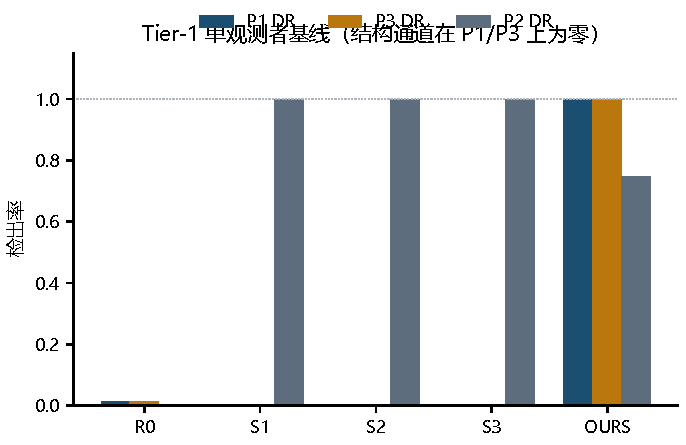
\includegraphics[width=\columnwidth]{fig/fig_tier1_CN.pdf}
  \Description{Bar chart of tier-1 baseline detection rates on P1 P2 P3.}
  \caption{第一档基线：单观测者方法族对 P1/P3 原理性失效，但对 P2 仍能发现沉默。}
  \label{fig:tier1}
\end{figure}

\begin{table}[t]
  \centering
  \caption{第一档基线（与本文采用相同窗口口径；判别力 ${=}$P1 DR${-}${FAR}）}
  \label{tab:tier1}
  \begin{tabular}{@{}lccccc@{}}
    \toprule
    方法 & FAR & P1 DR & P3 DR & P2 DR & 判别力 \\
    \midrule
    R0 随机指控 & 0.019 & 0.014 & 0.014 & 0.000 & $-0.005$ \\
    S1 看门狗 & 0.042 & 0.000 & 0.000 & 1.000 & $-0.042$ \\
    S2 计划残差 & 0.004 & 0.003 & 0.003 & 1.000 & $-0.001$ \\
    S3 过程一致性检验 & 0.000 & 0.000 & 0.000 & 1.000 & 0.000 \\
    \textbf{耦合互证} & 0.023 & \textbf{1.000} & \textbf{1.000} & 0.746 & \textbf{0.977} \\
    \bottomrule
  \end{tabular}
\end{table}

\subsection{第二档：见证选取原则（主结果）}
\label{sec:tier2}

本档实验采用同一互证协议、同一密码学构件、同一窗口与 260\,s 容差，仅替换见证选取策略 \texttt{WitnessPolicy}（图~\ref{fig:witness}、表~\ref{tab:tier2}）。
攻击参数与覆盖矩阵保持一致（攻击类型 P1，注入率 0.2，随机种子 42）。

\begin{figure*}[t]
  \centering
  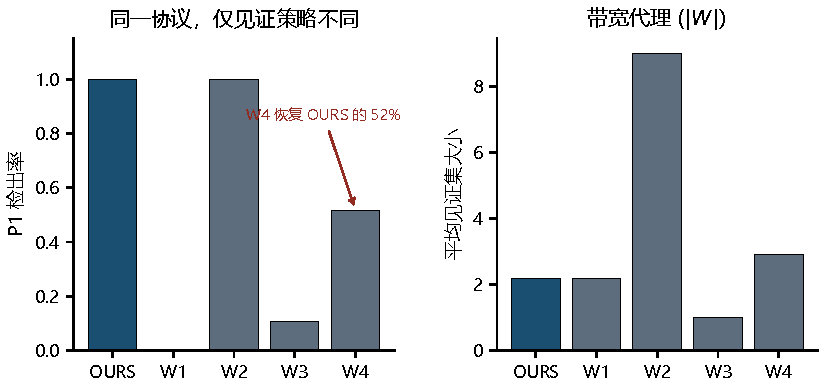
\includegraphics[width=0.88\textwidth]{fig/fig_witness_CN.pdf}
  \Description{P1 detection rate and mean witness set size for OURS and W1--W4.}
  \caption{第二档主结果：协议其余部分不变，仅替换见证选取策略。空间邻居策略（W4）只恢复 $0.518$ 的检出率，且见证集规模更大。}
  \label{fig:witness}
\end{figure*}

\begin{table}[t]
  \centering
  \caption{第二档：协议其余部分不变、仅替换见证选取策略（攻击类型 P1）}
  \label{tab:tier2}
  \small
  \begin{tabular}{@{}lccccc@{}}
    \toprule
    策略 & $\overline{|W|}$ & FAR & P1 DR & 判别力 & 未结算 \\
    \midrule
    \textbf{任务图对端设备} & 2.18 & 0.023 & \textbf{1.000} & \textbf{0.977} & 401 \\
    W1 法定人数 & 2.18 & 0.000 & 0.000 & 0.000 & 0 \\
    W2 全体询证 & 9.00 ($4.13\times$) & 0.023 & 1.000 & 0.977 & 900 \\
    W3 随机选取 $k$ 个 & 1.00 & 0.002 & 0.105 & 0.103 & 2\,162 \\
    W4 空间邻居 & 2.92 ($1.34\times$) & 0.000 & 0.518 & 0.518 & 1\,331 \\
    \bottomrule
  \end{tabular}
  \begin{tablenotes}
    \item W1 的 $\overline{|W|}$ 为协议见证集规模（不含共识副本）；其额外代价是全网共识消息带宽，约为沉默通道心跳带宽的 $131$ 倍。
  \end{tablenotes}
\end{table}

对表~\ref{tab:tier2} 的分析如下。
\begin{itemize}[leftmargin=*,itemsep=2pt]
  \item \textbf{W4（空间邻居）是主要对照。} 空间邻接关系是静态的，与当前流程实例实际所走的工艺路线无关；它只恢复 $0.518$ 的检出率，却多付出 $34\%$ 的见证集规模。这说明性能增量来自基于任务图的选取原则，而非见证者数量。
  \item \textbf{W1（法定人数）确认的是节点间消息一致，而非物理事实。} 其检出率恰为 $0$，能力等同于看门狗，而带宽约为本文的 $131$ 倍，即以高带宽代价换取了与看门狗相当的能力。实验中未向 W1 提供互证窗口与否证通道：若提供，它将额外获得约 $0.136$ 的检出率，这相当于把耦合互证机制本身赋予了它，从而不再构成对共识类方法的对照。
  \item \textbf{W2（全体询证）无任何增益。} 其检出率与误报率与本文完全一致，未结算条数由 401 增至 900 只是表面现象：双截止机制使从未被派发的候选见证者不会开启互证窗口，因此这些未结算项不会转化为错误指控。
  \item \textbf{W3（随机选取）的检出率降至 $0.105$。} 其失败模式是大量活动无法结算（2\,162 条），而非产生错误指控。
\end{itemize}
由此可见，``存在见证者''并不等同于``存在正确的见证者''。

\subsection{消融与覆盖矩阵}
\label{sec:ablation}

表~\ref{tab:coverage} 本身即为消融结果，对应热力图见图~\ref{fig:ablation}：移除互证通道后 P3 完全规避检测；移除沉默通道后 P1/P2 的检测时延恶化一至两个数量级。
两通道合用还带来另一项收益：在 P2 情形下，有 277 条诚实声明因其下游设备沉默而超时（良性流中仅 69 条）。
这并非协议的误报，而是攻击造成的真实后果——沉默设备同时拒绝为上游设备提供确认。
由于沉默通道能够直接判定出沉默设备，上游那些未获确认的声明才能被正确归因，而不致被误判为异常。

\begin{figure}[t]
  \centering
  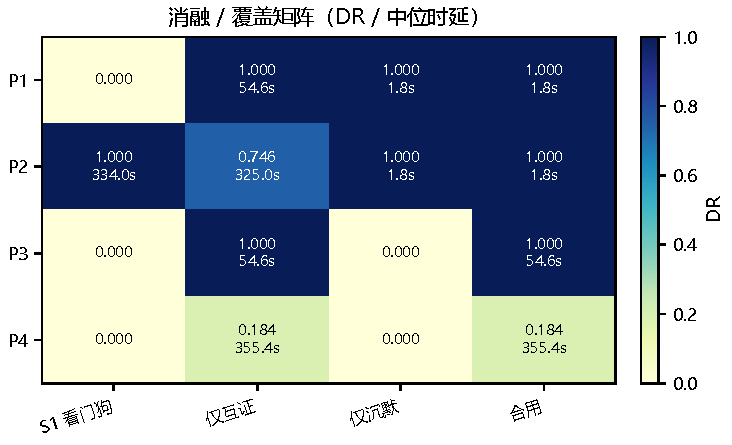
\includegraphics[width=\columnwidth]{fig/fig_ablation_CN.pdf}
  \Description{Heatmap of detection rate and latency across attacks and channels.}
  \caption{消融与覆盖矩阵热力图（格内为 DR 与时延中位数）。P3 行表明耦合互证不可替代。}
  \label{fig:ablation}
\end{figure}

\subsection{第三、四档与预算参数扫描}
\label{sec:tier34}

这两档不比较 P1 检出率（该指标在第一档中已是结构性零检出），其作用是衔接带宽定理并界定归责能力的边界。
在等带宽条件下，周期性全量上报（H1）的检测时延约为报文长度之比的 $8$ 倍（状态帧 128\,B 对原像 16\,B）；在最严格预算口径下，周期上报需 $4.68$\,s 才能判定沉默，而运动危害留给检测的时间仅为 $0.60$\,s——即在同等带宽下，该方案无法满足安全预算（图~\ref{fig:heartbeat}）。
H2/H3 与本文在归责能力上的差别见表~\ref{tab:h23}：GOOSE 式心跳具备活性检测能力，但无身份绑定，无法抵抗伪造心跳；TESLA 式延迟密钥在密钥披露后可由第三方重算 MAC，RFC~4082 亦明确声明其不提供不可否认性。
理想传感预言机（U1）的覆盖率为 $100\%$，相对本实现覆盖率的缺口约为 $29.95\%$（917 条；图~\ref{fig:coverage}），该值即第~\ref{sec:covdesign}~节所述按需探测目标区间的上界；本实现未插入探测动作，因此在该缺口上，若 P3 维持心跳则两通道合用仍无法检出。
沉默通道带宽相对 5\,Hz PBFT 的倍数关系见图~\ref{fig:budget-bw}；丢包率的参数扫描结果见图~\ref{fig:loss}（其中包含 $p{=}50\%$ 的参考点，突发丢包下约需 $27{,}502$\,B/s，仍为 PBFT 的 $1/36$）。

\begin{table}[t]
  \centering
  \caption{第三档：沉默检测与归责能力的边界界定（不比较 P1 检出率）}
  \label{tab:h23}
  \begin{tabular}{@{}lcccc@{}}
    \toprule
     & 发现沉默 & 身份绑定 & 披露后不可伪造 & 证据可转移 \\
    \midrule
    H1 等带宽周期上报 & 是（时延约 $8$ 倍） & --- & --- & --- \\
    H2 GOOSE 式心跳 & 是 & 否 & --- & 否 \\
    H3 TESLA 式延迟密钥 & 是 & 是 & \textbf{否} & 否 \\
    本文可问责沉默 & 是（上界 $r T_{\mathrm{hb}}$） & 承诺根签名 & 原像即一次性凭证 & 是 \\
    \bottomrule
  \end{tabular}
\end{table}

\begin{figure}[t]
  \centering
  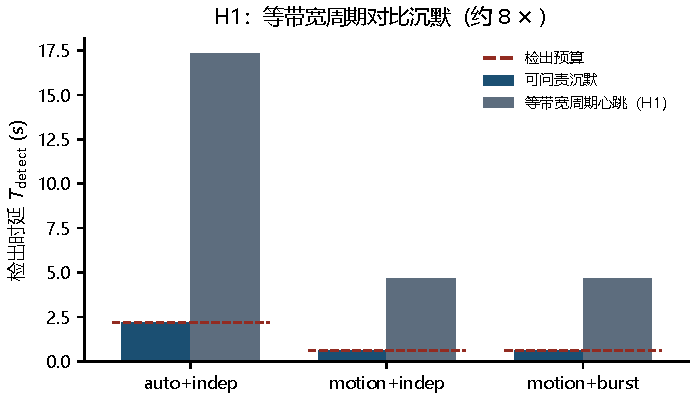
\includegraphics[width=\columnwidth]{fig/fig_heartbeat_CN.pdf}
  \Description{Equal-bandwidth periodic detection delay versus accountable silence.}
  \caption{第三档 H1：等带宽周期性全量上报的检测时延约为沉默通道的 $8$ 倍，且超出运动危害对应的检测预算。}
  \label{fig:heartbeat}
\end{figure}

\begin{figure}[t]
  \centering
  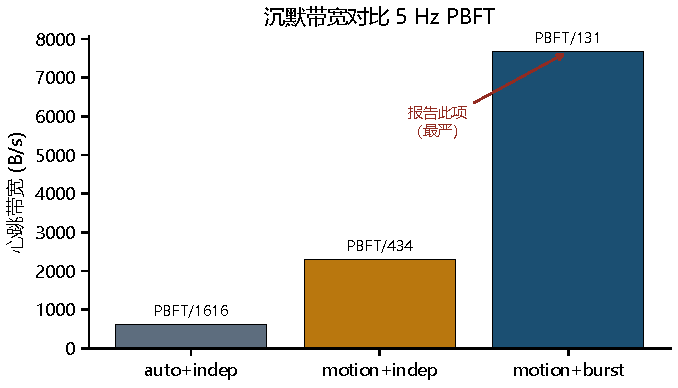
\includegraphics[width=\columnwidth]{fig/fig_budget_bw_CN.pdf}
  \Description{Silence heartbeat bandwidth under three regimes versus PBFT ratio.}
  \caption{可问责沉默的心跳带宽。本文报告最严格预算口径（运动危害 + 突发丢包，约为 PBFT 的 $1/131$）。}
  \label{fig:budget-bw}
\end{figure}

\begin{figure}[t]
  \centering
  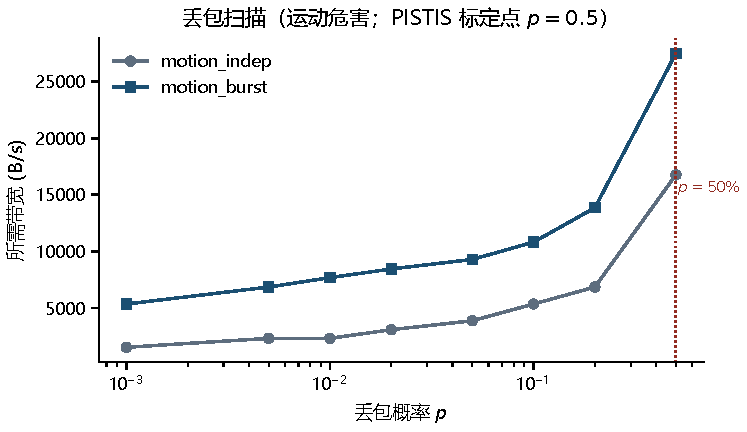
\includegraphics[width=\columnwidth]{fig/fig_loss_sweep_CN.pdf}
  \Description{Required bandwidth versus packet loss probability.}
  \caption{所需带宽随丢包率的变化（数据来源：\texttt{tessera/experiments/loss\_sweep.csv}）。}
  \label{fig:loss}
\end{figure}

\begin{figure}[t]
  \centering
  
\includegraphics[width=\columnwidth]{fig/fig_coverage_CN.pdf}
  \Description{Fraction of activities corroborated versus oracle gap.}
  \caption{第四档 U1：理想预言机覆盖率与本实现覆盖率之差（$29.95\%$）为按需探测目标区间的上界；本实现未插入探测动作。}
  \label{fig:coverage}
\end{figure}

%=============================================================================
\section{结论}
\label{sec:conclusion}

本文针对被劫持设备实施的无残差任务状态伪造，提出由任务图诱导的耦合互证，以及不依赖共识分歧的可问责沉默，并将心跳间隔与危害模型导出的时间预算相衔接。

\subsection{结论与贡献}
\label{sec:contributions}

存在对端设备时，两通道合用后 P1--P3 均不存在可行的获胜分支；在缺乏对端设备的覆盖缺口上，P3 仍可规避检测。
Trier 数据集上的实验结论如下：单观测者方法族对 P1/P3 原理性失效；在协议其余部分不变、仅替换见证选取策略时，空间邻居策略只恢复 $0.518$ 的检出率；P3 的结果说明耦合互证不可替代；在 $n{=}28$ 的对照规模下，最严格预算口径下的心跳带宽为 $7.7$\,KB/s，约为 5\,Hz 全网 PBFT 的 $1/131$。
部署层面的含义是：$T_{\mathrm{hb}}$ 应由安全时间预算反向求解得出，见证集应依据任务图配置。

\subsection{局限}
\label{sec:discussion}

W4 仅恢复约一半检出率，原因在于空间邻接关系与当前工件实际所走的工艺路线无关：它既遗漏了在任务图上相邻、但在空间上不相邻的真实对端设备，又纳入了大量无关设备；而本文的选取规则由任务图与当前流程实例共同确定，具有动态性。
$29.95\%$ 的覆盖缺口并非实现上的缺陷：每个流程实例的末位活动没有下游设备接手，这构成结构性上界；剔除末位活动后，链内覆盖率约为 $77\%$。
其余缺口（入库后无设备接手、同一设备原地完成多道工步）无法通过排产调整消除，本实现亦未插入主动探测，因此这些区间上的完成类伪造不在互证覆盖范围内：若 P3 维持心跳，则该分支获胜。
传感能力不足是另一项部署约束：当存在对端设备但不具备到料、取件传感时，P1 只能依靠逾窗判定，检出率降至 $0.860$，时延中位数约为 $365$\,s；主表中的 $1.000/54.6$ 对应具备传感能力的口径。

运动危害下的 FHI 仅用于校准心跳预算的量级；本文考虑的主要危害仍是调度损害（伪报完成或空闲、造成下游工位饥饿等），不应将 ISO 距离公式解读为已经证明了碰撞安全性。
一跳串谋是定义~\ref{def:closure} 所量化的结构性边界，而非检测遗漏：伪造的任务状态若要维持到物料被消耗，攻击者须控制前向可达闭包上的每一跳设备；其中 $k_{\min}{=}1$ 的 23 条链必须如实报告。

其他局限包括：方法要求松散时间同步与有界心跳，否则归责将退化为异步系统中的不可归因问题；由于不假设 TEE，方法不检测软件篡改本身，只检测其在任务状态上的外显后果；FHI、丢包率与突发相关系数均非 Trier 日志的实测值；主实验仅基于单一日志，且未对注入率与随机种子作参数扫描。

\subsection{未来工作}
\label{sec:future}

针对上述局限，后续工作包括：在柔性车间中引入低成本的可观测动作，以弥补缺乏对端设备的覆盖缺口并提高 $k_{\min}$；在真实网络环境中标定丢包率与时间同步精度；对注入率与随机种子开展参数扫描实验。

\begin{acks}
感谢 Fischertechnik Trier 事件日志的维护者提供公开数据~\cite{trier2022}。
原型 TESSERA 与配套断言集随本文开源。
\end{acks}

\paragraph{数据与代码可用性。}
协议、各基线与攻击注入器均实现于开源原型 TESSERA（\texttt{paper03/tessera}）。
复现入口为 \texttt{py main.py}；断言集 \texttt{tests/test\_all.py}（共 63 条）用于锚定本文主表结果。
主数据为公开的 Trier IoT 事件日志与配套的 16 个 BPMN 模型~\cite{trier2022}。

%=============================================================================
\appendix
\section{命题~\ref{prop:nr} 的归约证明}
\label{app:nr}

记单向哈希函数为 $H:\{0,1\}^\ast\to\{0,1\}^\lambda$（实现中取 $\lambda{=}128$，要求原像抗性；域分离标签 $\mathsf{tessera}|\mathrm{id}|\mathrm{session}$ 参与每一步哈希计算）。
设备 $d$ 抽取随机种子并构造反向哈希链，令 $h_0$ 为承诺根，再用 Ed25519 私钥计算
$\sigma\leftarrow\mathrm{Sign}_{sk}(\langle\mathrm{id},\,\mathrm{session},\,h_0,\,N,\,t_0,\,T_{\mathrm{hb}}\rangle)$，
并以 $R_d=(h_0,\sigma)$ 完成注册。
槽 $k$ 的合法凭证是满足 $H^{(k)}(h_k)=h_0$ 的 $h_k$；验证者拒绝在槽 $k$ 尚未截止时到达的 $h_{k'}$（$k'>k$）。

\textbf{验证过程。}
第三方在持有 $R_d$ 与 $h_k$ 时检查如下三项：（i）$\sigma$ 在公钥 $pk$ 下对上述绑定内容验证通过；（ii）带域分离的 $H^{(k)}(h_k)=h_0$ 成立；（iii）披露时刻 $\le t_k^\star=t_0+k T_{\mathrm{hb}}+\varepsilon$。
三项同时成立则接受``$d$ 在槽 $k$ 披露过原像''这一结论（不可否认的是原像来源，并不蕴含任务状态为真）。

\textbf{伪造游戏。}
敌手 $\mathcal{A}$ 不持有随机种子与私钥 $sk$，但可自适应地观察截止时刻之前的合法披露 $\{h_j\}_{j<k}$，并输出 $(k^\star,h^\star)$。
若该输出通过验证，且 $h^\star$ 并非 $d$ 在槽 $k^\star$ 的合法原像，则 $\mathcal{A}$ 获胜。
以下分两种类型讨论：

\emph{类型 I（原像）。}
绑定字段与 $R_d$ 一致，但 $h^\star$ 满足 $H^{(k^\star)}(h^\star)=h_0$ 且 $h^\star\neq h_{k^\star}$。
此时 $h^\star$ 构成对 $H^{(k^\star)}(\cdot)=h_0$ 的第二原像（或在已知后缀 $h_j$、$j<k^\star$ 的情况下构成对下一步 $H$ 的原像）。
由 $H$ 的单向性，该事件的发生概率可忽略。
已披露的 $h_j$（$j<k^\star$）无法前向推出 $h_{k^\star}$，因为哈希链按反向生成；而提前披露 $h_{k^\star+1}$ 会被协议拒绝，故攻击者无法为未来的槽预先取得凭证。

\emph{类型 II（篡改绑定）。}
$\mathcal{A}$ 输出对应另一身份、或另一组 $(N,t_0,T_{\mathrm{hb}})$ 的承诺根 $R'$，并使验证通过。
此时 $\mathcal{A}$ 即给出了对 Ed25519 的 EUF-CMA 伪造。

与 TESLA~\cite{tesla2001,rfc4082} 的差别在于：TESLA 将链元素用作 MAC 密钥，密钥披露后任何人均可重算 MAC；而此处的凭证本身即为原像，其披露不会产生可用于冒充消息源的对称密钥。
因此，在条件（i）--（iii）下，在截止时刻之后伪造合法的 $h_k$ 可归约为打破 $H$ 的单向性或伪造 Ed25519 签名。

%=============================================================================
\begin{thebibliography}{99}

\bibitem{pistis2021}
D.~Kozhaya, J.~Decouchant, and P.~Esteves-Verissimo,
``PISTIS: An Event-Triggered Real-Time Byzantine-Resilient Protocol Suite,''
\textit{IEEE Trans. Parallel Distrib. Syst.}, vol.~32, no.~9, pp.~2271--2286, 2021.

\bibitem{tac2025el}
``Event-Triggered Resilient Consensus of Networked Euler--Lagrange Systems Under Byzantine Attacks,''
\textit{IEEE Trans. Autom. Control}, 2025, doi:10.1109/TAC.2025.3582531.

\bibitem{hdetm2024}
``A robust control framework for multi-agent systems under Byzantine attacks using hybrid event-triggered techniques,''
\textit{Ain Shams Eng. J.}, 2024, doi:10.1016/j.asej.2024.103149.

\bibitem{ccgridw2023pbft}
``An Improved PBFT-Based Consensus Protocol for Industrial IoT,''
in \textit{Proc. CCGridW}, 2023, doi:10.1109/CCGridW59191.2023.00068.

\bibitem{sensors2024aloha}
``Slotted ALOHA Based PBFT Blockchain Networks: Performance Analysis and Optimization,''
\textit{Sensors}, vol.~24, no.~23, p.~7688, 2024.

\bibitem{nontrigger2022}
``Performance Analysis of Event-Triggered Consensus Control for Multi-agent Systems under Cyber-Physical Attacks,''
\textit{arXiv:2201.02997}, 2022.

\bibitem{asjc2023contain}
``Event-triggered containment control for multi-agent systems under hybrid cyber attacks,''
\textit{Asian J. Control}, 2023, doi:10.1002/asjc.3180.

\bibitem{ijrnc2023deception}
``Event-triggered control of Takagi--Sugeno fuzzy systems under deception attacks,''
\textit{Int. J. Robust Nonlinear Control}, 2023, doi:10.1002/rnc.6760.

\bibitem{peerreview2007}
A.~Haeberlen, P.~Kuznetsov, and P.~Druschel,
``PeerReview: Practical Accountability for Distributed Systems,''
in \textit{Proc. SOSP}, 2007, pp.~175--188.

\bibitem{polygraph2021}
P.~Civit, S.~Gilbert, and V.~Gramoli,
``Polygraph: Accountable Byzantine Agreement,''
in \textit{Proc. ICDCS}, 2021, pp.~403--413.

\bibitem{abc2023}
P.~Civit, S.~Gilbert, V.~Gramoli, et~al.,
``As easy as ABC: Optimal Accountable Byzantine Consensus is easy!,''
\textit{J. Parallel Distrib. Comput.}, vol.~181, 2023.

\bibitem{tesla2001}
A.~Perrig, R.~Canetti, J.~D.~Tygar, and D.~Song,
``Efficient Authentication and Signing of Multicast Streams over Lossy Channels,''
in \textit{Proc. IEEE Symp. Security and Privacy}, 2000.

\bibitem{rfc4082}
A.~Perrig, D.~Song, R.~Canetti, J.~D.~Tygar, and B.~Briscoe,
``Timed Efficient Stream Loss-Tolerant Authentication (TESLA),''
RFC~4082, 2005.

\bibitem{inftesla2022}
``Enhanced Inf-TESLA Protocol,''
\textit{IEEE Access}, 2022, doi:10.1109/ACCESS.2022.3177268.

\bibitem{goose615}
ABB,
``IEC 61850 Engineering Guide: 615 series,''
technical manual (GOOSE MaxTime / TAL heartbeat semantics).

\bibitem{diat2019}
T.~Abera, R.~Bahmani, F.~Brasser, et~al.,
``DIAT: Data Integrity Attestation for Resilient Collaboration of Autonomous Systems,''
in \textit{Proc. NDSS}, 2019.

\bibitem{colaw2020}
P.~Barabas, E.~Regnath, and S.~Steinhorst,
``COLAW: Cooperative Location Proof Architecture for VANETs based on Witnessing,''
in \textit{Proc. COINS}, 2020, doi:10.1109/COINS49042.2020.9191402.

\bibitem{vouch2019}
F.~Boeira, M.~Asplund, and M.~Barcellos,
``Decentralized proof of location in vehicular ad hoc networks,''
\textit{Comput. Commun.}, vol.~147, pp.~98--110, 2019.

\bibitem{etsi460}
ETSI,
``Intelligent Transport Systems; Security; Pre-standardization study on Misbehaviour Detection,''
ETSI TR 103 460 V2.1.1.

\bibitem{ditof2024}
J.~Bahrami, M.~Ebrahimabadi, M.~Younis, and N.~Karimi,
``Digital Twin Based Topology Fingerprinting for Detecting False Data Injection Attacks in Cyber-Physical Systems,''
in \textit{Proc. IEEE ICC}, 2024, pp.~2053--2058.

\bibitem{dtmpc2025}
``Digital Twin-Based Resilient Model Predictive Control for Industrial Cyber-Physical Systems,''
\textit{IEEE J. Emerg. Sel. Topics Ind. Electron.}, 2025, doi:10.1109/JESTIE.2025.3528881.

\bibitem{agvkpi2022}
``Detecting and Processing Anomalies in a Factory of the Future,''
\textit{Appl. Sci.}, vol.~12, no.~16, p.~8181, 2022.

\bibitem{fdi2024frontiers}
``An evaluation of methods for detecting false data injection attacks in the smart grid,''
\textit{Frontiers Comput. Sci.}, 2024.

\bibitem{cn120578205b}
``一种抗虚假数据注入攻击的多 AGV 事件触发安全路径跟踪方法,''
中国专利 CN120578205B.

\bibitem{usaid}
A.~Ibrahim, A.-R.~Sadeghi, and G.~Tsudik,
``US-AID: Unattended Scalable Attestation of IoT Devices,''
in \textit{Proc. IEEE SRDS}, 2018, pp.~21--30.

\bibitem{trier2022}
L.~Malburg, J.~Gr\"uger, and R.~Bergmann,
``An IoT-Enriched Event Log for Process Mining in Smart Factories,''
\textit{arXiv:2209.02702}, 2022.

\bibitem{iso13855}
ISO~13855,
``Safety of machinery --- Positioning of safeguards with respect to the approach speeds of parts of the human body.''

\bibitem{iso3691}
ISO~3691-4:2023,
``Industrial trucks --- Safety requirements and verification --- Part~4: Driverless industrial trucks.''

\bibitem{ase2023fhi}
J.~S.~Becker, B.~Koopmann, I.~Stierand, and L.~Westhofen,
``Providing Evidence for Correct and Timely Functioning of Software Safety Mechanisms,''
in \textit{Proc. Software Engineering 2023 Workshops}, 2023, pp.~66--77, doi:10.18420/se2023-ws-09.

\end{thebibliography}

\end{document}
